        %%******************************************%%
        %%                                          %%
        %%        Modello di tesi di laurea         %%
        %%            di Andrea Giraldin            %%
        %%                                          %%
        %%             2 novembre 2012              %%
        %%                                          %%
        %%******************************************%%


% I seguenti commenti speciali impostano:
% 1. 
% 2. PDFLaTeX come motore di composizione;
% 3. tesi.tex come documento principale;
% 4. il controllo ortografico italiano per l'editor.

% !TEX encoding = UTF-8
% !TEX TS-program = pdflatex
% !TEX root = tesi.tex
% !TEX spellcheck = it-IT

\documentclass[10pt,                    % corpo del font principale
               a4paper,                 % carta A4
               twoside,                 % impagina per fronte-retro
               openright,               % inizio capitoli a destra
               english,                 
               italian,                 
               ]{book}    

%**************************************************************
% Importazione package
%************************************************************** 

%\usepackage{amsmath,amssymb,amsthm}    % matematica

\usepackage[T1]{fontenc}                % codifica dei font:
                                        % NOTA BENE! richiede una distribuzione *completa* di LaTeX

\usepackage{lmodern}

\usepackage[utf8]{inputenc}             % codifica di input; anche [latin1] va bene
                                        % NOTA BENE! va accordata con le preferenze dell'editor

\usepackage[english, italian]{babel}    % per scrivere in italiano e in inglese;
                                        % l'ultima lingua (l'italiano) risulta predefinita


\usepackage{bookmark}                   % segnalibri

\usepackage{caption}                    % didascalie

\usepackage{chngpage,calc}              % centra il frontespizio

\usepackage{csquotes}                   % gestisce automaticamente i caratteri (")

\usepackage{emptypage}                  % pagine vuote senza testatina e piede di pagina

\usepackage{epigraph}			% per epigrafi

\usepackage{eurosym}                    % simbolo dell'euro

%\usepackage{indentfirst}               % rientra il primo paragrafo di ogni sezione

\usepackage{graphicx}                   % immagini

\usepackage{hyperref}                   % collegamenti ipertestuali

\usepackage[binding=5mm]{layaureo}      % margini ottimizzati per l'A4; rilegatura di 5 mm

\usepackage{listings}                   % codici

\usepackage{microtype}                  % microtipografia

\usepackage{mparhack,fixltx2e,relsize}  % finezze tipografiche

\usepackage{nameref}                    % visualizza nome dei riferimenti                                      

\usepackage[font=small]{quoting}        % citazioni

\usepackage{subfig}                     % sottofigure, sottotabelle

\usepackage[italian]{varioref}          % riferimenti completi della pagina

\usepackage{booktabs}                   % tabelle                                       
\usepackage{tabularx}                   % tabelle di larghezza prefissata                                    
\usepackage{longtable}                  % tabelle su più pagine                                        
\usepackage{ltxtable}                   % tabelle su più pagine e adattabili in larghezza
\renewcommand\arraystretch{1.5}
\usepackage[toc, acronym]{glossaries}   % glossario
                                        % per includerlo nel documento bisogna:
                                        % 1. compilare una prima volta tesi.tex;
                                        % 2. eseguire: makeindex -s tesi.ist -t tesi.glg -o tesi.gls tesi.glo
                                        % 3. eseguire: makeindex -s tesi.ist -t tesi.alg -o tesi.acr tesi.acn
                                        % 4. compilare due volte tesi.tex.

\usepackage[backend=biber,style=verbose-ibid,hyperref,backref]{biblatex}
                                        % eccellente pacchetto per la bibliografia; 
                                        % produce uno stile di citazione autore-anno; 
                                        % lo stile "numeric-comp" produce riferimenti numerici
                                        % per includerlo nel documento bisogna:
                                        % 1. compilare una prima volta tesi.tex;
                                        % 2. eseguire: biber tesi
                                        % 3. compilare ancora tesi.tex.

%**************************************************************
% file contenente le impostazioni della tesi
%**************************************************************

%**************************************************************
% Frontespizio
%**************************************************************

% Autore
\newcommand{\myName}{Marco Rampazzo}                                    
\newcommand{\myTitle}{Metodologie agili applicate allo sviluppo di una componente d'interfaccia grafica web in Kotlin per l'analisi di Big Data}

% Tipo di tesi                   
\newcommand{\myDegree}{Tesi di laurea}

% Università             
\newcommand{\myUni}{Università degli Studi di Padova}

% Facoltà       
\newcommand{\myFaculty}{Corso di Laurea in Informatica}

% Dipartimento
\newcommand{\myDepartment}{Dipartimento di Matematica "Tullio Levi-Civita"}

% Titolo del relatore
\newcommand{\profTitle}{Prof. }

% Relatore
\newcommand{\myProf}{Claudio Enrico Palazzi}

% Luogo
\newcommand{\myLocation}{Padova}

% Anno accademico
\newcommand{\myAA}{2019-2020}

% Data discussione
\newcommand{\myTime}{Dicembre 2020}


%**************************************************************
% Impostazioni di impaginazione
% see: http://wwwcdf.pd.infn.it/AppuntiLinux/a2547.htm
%**************************************************************

\setlength{\parindent}{14pt}   % larghezza rientro della prima riga
\setlength{\parskip}{0pt}   % distanza tra i paragrafi


%**************************************************************
% Impostazioni di biblatex
%**************************************************************
\bibliography{bibliografia} % database di biblatex 


\defbibheading{bibliography} {
    \cleardoublepage
    \phantomsection 
    \addcontentsline{toc}{chapter}{\bibname}
    \chapter*{\bibname\markboth{\bibname}{\bibname}}
}

\setlength\bibitemsep{1.5\itemsep} % spazio tra entry

\DeclareBibliographyCategory{opere}
\DeclareBibliographyCategory{web}

\addtocategory{opere}{womak:lean-thinking}
\addtocategory{web}{site:agile-manifesto}

\defbibheading{opere}{\section*{Riferimenti bibliografici}}
\defbibheading{web}{\section*{Siti Web consultati}}


%**************************************************************
% Impostazioni di caption
%**************************************************************
\captionsetup{
    tableposition=top,
    figureposition=bottom,
    font=small,
    format=hang,
    labelfont=bf
}

%**************************************************************
% Impostazioni di glossaries
%**************************************************************

%**************************************************************
% Acronimi
%**************************************************************
\renewcommand{\acronymname}{Acronimi e abbreviazioni}

\newacronym[description={\glslink{apig}{Application Program Interface}}]
    {api}{API}{Application Program Interface}

\newacronym[description={\glslink{umlg}{Unified Modeling Language}}]
    {uml}{UML}{Unified Modeling Language}

%**************************************************************
% Glossario
%**************************************************************
%\renewcommand{\glossaryname}{Glossario}

\newglossaryentry{apig}
{
    name=\glslink{api}{API},
    text=Application Program Interface,
    sort=api,
    description={in informatica con il termine \emph{Application Programming Interface API} (ing. interfaccia di programmazione di un'applicazione) si indica ogni insieme di procedure disponibili al programmatore, di solito raggruppate a formare un set di strumenti specifici per l'espletamento di un determinato compito all'interno di un certo programma. La finalità è ottenere un'astrazione, di solito tra l'hardware e il programmatore o tra software a basso e quello ad alto livello semplificando così il lavoro di programmazione}
}


\newglossaryentry{dataflowg}
{
    name=Dataflow,
    text=dataflow,
    sort=dataflow,
    description={Il dataflow è un paradigma di programmazione basato sull'idea di disconnettere gli attori computazionali in "pipelines" che possono eseguire azioni in modo concorrente. Nell'ambito di questo progetto usando "dataflow" si intende il modo in cui i dati vengono trasmessi tra gli attori computazionali}
}

\newglossaryentry{webappg}
{
	name=Web App,
	text=Web App,
	sort=webapp,
	description={Una applicazione web (o web app) è un software che viene eseguito su un web server. Rispetto ad applicazioni che vengono eseguite localmente sul sistema operativo, le applicazioni web possono essere eseguite da un utente mediante un browser e una connessione internet}
}

\newglossaryentry{scrumg}
{
	name=SCRUM,
	text=SCRUM,
	sort=scrum,
	description={Scrum è un framework agile per lo sviluppo e la distribuzione e la manutenzione di prodotti complessi. Esso è stato realizzato per team di sviluppo ristretti (meno di 10 membri) che dividino il loro lavoro in obiettivi che possono essere completati all'interno di iterazioni con un tempo limitato che si chiamano "sprint". Alla fine di uno "sprint" il team di sviluppo partecipa alla riunione di "sprint review" per dimostrare il lavoro fatto, infine uno "sprint retrospective" per ottenere un miglioramento continuo}
}

\newglossaryentry{hofg}
{
	name=Funzioni di ordine superiore / Higher order functions,
	text=Funzioni di ordine superiore / Higher order functions,
	sort=hofg,
	description={
		In matematica ed in informatica, una funzione di ordine superiore (o higher order function) è una funzione che presenta almeno una di queste caratteristiche:
		\begin{itemize}
			\item accetta come argomento una o più funzioni (parametri procedurali);
			\item ritorna una funzione come risultato.
		\end{itemize}
		Un esempio nella matematica è l'operatore di derivazione dato che viene mappata una funzione ad un'altra funzione}
}

\newglossaryentry{sideeffectsg}
{
	name=Side effects,
	text=Side effects,
	sort=sideeffects,
	description={In informatica una funziona, operazione o espressione viene detta di avere "side effect" se modifica variabili di stato al di fuori del suo ambiente locale. In particolare se c'è un effetto osservabile al di fuori del valore che viene ritornato ("main effect") all'invocatore della funzione, operazione o espressione}
}

\newglossaryentry{vcsg}
{
	name=VCS,
	text=VCS,
	sort=vcs,
	description={VCS o "Version Control System". In ingegneria del software, il controllo del versionamento è una classe di sistemi responsabili della gestione di cambiamenti nel codice sorgente di un software. Ogni cambiamento (revisione) viene identificato attraverso un numero o un codice, esso viene associato ad un'orario e alla persona che ha eseguito la modifica. Ogni revisione può essere confrontata, restaurata e, con alcuni tipi di file, combinata (merged)}
}

\newglossaryentry{itsg}
{
	name=ITS,
	text=ITS,
	sort=its,
	description={ITS o "Issue Tracking System" è un pacchetto software che si occupa di gestire e mantenere una lista di attività (issues) da completare. Un ITS viene utilizzato principalmente durante la collaborazione in team di sviluppo grandi, tuttavia può essere utilizzato da individui per gestire il proprio tempo e/o la loro produttività}
}

\newglossaryentry{ideg}
{
	name=IDE,
	text=IDE,
	sort=ide,
	description={IDE o "Integrated Development Environment" è un software per sviluppare applicazioni che combina strumenti per lo sviluppatore in un'interfaccia grafica comune}
}

\newglossaryentry{buildautomationg}
{
	name=Build automation,
	text=Build automation,
	sort=buildautomation,
	description={Con Build automation si intende il processo di automatizzare la creazione di un software e i processi associati ad esso tra i quali: compilazione del codice sorgente, esecuzione di test automatici e il "packaging" del codice binario risultante}
}

\newglossaryentry{purefunctionsg}
{
	name=Funzioni pure,
	text=Funzioni pure,
	sort=purefunctions,
	description={Una funzione è definita come "pura" quando il valore di output è determinato solamente dall'input della funzione senza nessun "side effect" osservabile}
}

\newglossaryentry{propsg}
{
	name=Props,
	text=Props,
	sort=props,
	description={I componenti di React sono delle funzioni Javascript, esse accettano dei valori di input chiamati "props". Quindi le "props" sono i dati che possono essere passati come argomento ad un componente React}
}



 % database di termini
\makeglossaries


%**************************************************************
% Impostazioni di graphicx
%**************************************************************
\graphicspath{{immagini/}} % cartella dove sono riposte le immagini


%**************************************************************
% Impostazioni di hyperref
%**************************************************************
\hypersetup{
    %hyperfootnotes=false,
    %pdfpagelabels,
    %draft,	% = elimina tutti i link (utile per stampe in bianco e nero)
    colorlinks=true,
    linktocpage=true,
    pdfstartpage=1,
    pdfstartview=FitV,
    % decommenta la riga seguente per avere link in nero (per esempio per la stampa in bianco e nero)
    %colorlinks=false, linktocpage=false, pdfborder={0 0 0}, pdfstartpage=1, pdfstartview=FitV,
    breaklinks=true,
    pdfpagemode=UseNone,
    pageanchor=true,
    pdfpagemode=UseOutlines,
    plainpages=false,
    bookmarksnumbered,
    bookmarksopen=true,
    bookmarksopenlevel=1,
    hypertexnames=true,
    pdfhighlight=/O,
    %nesting=true,
    %frenchlinks,
    urlcolor=webbrown,
    linkcolor=RoyalBlue,
    citecolor=webgreen,
    %pagecolor=RoyalBlue,
    %urlcolor=Black, linkcolor=Black, citecolor=Black, %pagecolor=Black,
    pdftitle={\myTitle},
    pdfauthor={\textcopyright\ \myName, \myUni, \myFaculty},
    pdfsubject={},
    pdfkeywords={},
    pdfcreator={pdfLaTeX},
    pdfproducer={LaTeX}
}
\setcounter{secnumdepth}{3}
\setcounter{tocdepth}{3}
\usepackage{listings}
\usepackage{dirtree}
\usepackage[dvipsnames, rgb, x11names, html]{xcolor}
\usepackage{courier}

\colorlet{punct}{red!60!black}
\definecolor{background}{HTML}{FFFFFF}
\definecolor{delim}{RGB}{20,105,176}
\colorlet{numb}{magenta!60!black}

\lstdefinelanguage{json}{
	basicstyle=\footnotesize\ttfamily,
	numbers=left,
	numberstyle=\footnotesize,
	stepnumber=1,
	numbersep=8pt,
	showstringspaces=false,
	breaklines=true,
	frame=lines,
	backgroundcolor=\color{background},
	literate=
	*{0}{{{\color{numb}0}}}{1}
	{1}{{{\color{numb}1}}}{1}
	{2}{{{\color{numb}2}}}{1}
	{3}{{{\color{numb}3}}}{1}
	{4}{{{\color{numb}4}}}{1}
	{5}{{{\color{numb}5}}}{1}
	{6}{{{\color{numb}6}}}{1}
	{7}{{{\color{numb}7}}}{1}
	{8}{{{\color{numb}8}}}{1}
	{9}{{{\color{numb}9}}}{1}
	{:}{{{\color{punct}{:}}}}{1}
	{,}{{{\color{punct}{,}}}}{1}
	{\{}{{{\color{delim}{\{}}}}{1}
	{\}}{{{\color{delim}{\}}}}}{1}
	{[}{{{\color{delim}{[}}}}{1}
	{]}{{{\color{delim}{]}}}}{1},
}

\lstdefinelanguage{Kotlin}{
	comment=[l]{//},
	emph={delegate, filter, first, firstOrNull, forEach, lazy, map, mapNotNull, println, return@, abstract, actual, as, as?, break, by, class, companion, continue, data, do, dynamic, else, enum, expect, false, final, for, fun, get, if, import, in, interface, internal, is, null, object, override, package, private, public, return, set, super, suspend, this, throw, true, try, typealias, val, var, vararg, when, where, while},
	keywords={DimensionsNode, TableState, NodeActionType, HeaderAction, BodyCells},
	numbers=left,
	numberstyle=\scriptsize,
	stepnumber=1,
	numbersep=8pt,
	showstringspaces=false,
	frame=lines,
	morecomment=[s]{/*}{*/},
	morestring=[b]",
	morestring=[s]{"""*}{*"""},
	ndkeywords={@Deprecated, @JvmField, @JvmName, @JvmOverloads, @JvmStatic, @JvmSynthetic, Array, Byte, Double, Float, Int, Integer, Iterable, Long, Runnable, Short, String, ArrayList, List, Int?},
	sensitive=true,
	backgroundcolor=\color{sbase3},
	basicstyle=\color{sbase00}\footnotesize\ttfamily,
	keywordstyle=\color{sorange},
	commentstyle=\color{sbase1},
	stringstyle=\color{sblue},
	numberstyle=\color{sviolet},
	emphstyle=\color{sviolet},
	identifierstyle=\color{sbase00},
}

%**************************************************************
% Impostazioni di itemize
%**************************************************************
%\renewcommand{\labelitemi}{$\ast$}

\renewcommand{\labelitemi}{$\bullet$}
%\renewcommand{\labelitemii}{$\cdot$}
%\renewcommand{\labelitemiii}{$\diamond$}
%\renewcommand{\labelitemiv}{$\ast$}


%**************************************************************
% Impostazioni di listings
%**************************************************************
\lstset{
    language=[LaTeX]Tex,%C++,
    keywordstyle=\color{RoyalBlue}, %\bfseries,
    basicstyle=\small\ttfamily,
    %identifierstyle=\color{NavyBlue},
    commentstyle=\color{Green}\ttfamily,
    stringstyle=\rmfamily,
    numbers=none, %left,%
    numberstyle=\scriptsize, %\tiny
    stepnumber=5,
    numbersep=8pt,
    showstringspaces=false,
    breaklines=true,
    frameround=ftff,
    frame=single
} 


%**************************************************************
% Impostazioni di xcolor
%**************************************************************
\definecolor{webgreen}{rgb}{0,.5,0}
\definecolor{webbrown}{rgb}{.6,0,0}
\definecolor{sbase03}{HTML}{002B36}
\definecolor{sbase02}{HTML}{073642}
\definecolor{sbase01}{HTML}{586E75}

\definecolor{sbase0}{HTML}{839496}
\definecolor{sbase1}{HTML}{93A1A1}
\definecolor{sbase2}{HTML}{EEE8D5}

\definecolor{syellow}{HTML}{B58900}
\definecolor{sorange}{HTML}{CB4B16}
\definecolor{sred}{HTML}{DC322F}
\definecolor{smagenta}{HTML}{D33682}
\definecolor{sviolet}{HTML}{6C71C4}
\definecolor{sblue}{HTML}{268BD2}
\definecolor{scyan}{HTML}{2AA198}
\definecolor{sgreen}{HTML}{859900}

\definecolor{sbase00}{HTML}{000000}
\definecolor{sbase3}{HTML}{FFFFFF}

%**************************************************************
% Altro
%**************************************************************

\newcommand{\omissis}{[\dots\negthinspace]} % produce [...]

% eccezioni all'algoritmo di sillabazione
\hyphenation
{
    ma-cro-istru-zio-ne
    gi-ral-din
}

\newcommand{\sectionname}{sezione}
\addto\captionsitalian{\renewcommand{\figurename}{Figura}
                       \renewcommand{\tablename}{Tabella}}

\newcommand{\glsfirstoccur}{\ap{{[g]}}}

\newcommand{\glo}{$_G$} %Comando per aggiungere il pedice G
\newcommand{\glosp}{$_G$ } %Comando per aggiungere il pedice G con spazio

\newcommand{\intro}[1]{\emph{\textsf{#1}}}

%**************************************************************
% Environment per ``rischi''
%**************************************************************
\newcounter{riskcounter}                % define a counter
\setcounter{riskcounter}{0}             % set the counter to some initial value

%%%% Parameters
% #1: Title
\newenvironment{risk}[1]{
    \refstepcounter{riskcounter}        % increment counter
    \par \noindent                      % start new paragraph
    \textbf{\arabic{riskcounter}. #1}   % display the title before the 
                                        % content of the environment is displayed 
}{
    \par\medskip
}

\newcommand{\riskname}{Rischio}

\newcommand{\riskdescription}[1]{\textbf{\\Descrizione:} #1.}

\newcommand{\risksolution}[1]{\textbf{\\Soluzione:} #1.}

%**************************************************************
% Environment per ``use case''
%**************************************************************
\newcounter{usecasecounter}             % define a counter
\setcounter{usecasecounter}{0}          % set the counter to some initial value

%%%% Parameters
% #1: ID
% #2: Nome
\newenvironment{usecase}[2]{
    \renewcommand{\theusecasecounter}{\usecasename #1}  % this is where the display of 
                                                        % the counter is overwritten/modified
    \refstepcounter{usecasecounter}             % increment counter
    \vspace{10pt}
    \par \noindent                              % start new paragraph
    {\large \textbf{\usecasename #1: #2}}       % display the title before the 
                                                % content of the environment is displayed 
    \medskip
}{
    \medskip
}

\newcommand{\usecasename}{UC}

\newcommand{\usecaseactors}[1]{\textbf{\\Attori Principali:} #1. \vspace{4pt}}
\newcommand{\usecasepre}[1]{\textbf{\\Precondizioni:} #1. \vspace{4pt}}
\newcommand{\usecasedesc}[1]{\textbf{\\Descrizione:} #1. \vspace{4pt}}
\newcommand{\usecasepost}[1]{\textbf{\\Postcondizioni:} #1. \vspace{4pt}}
\newcommand{\usecasealt}[1]{\textbf{\\Scenario Alternativo:} #1. \vspace{4pt}}

%**************************************************************
% Environment per ``namespace description''
%**************************************************************

\newenvironment{namespacedesc}{
    \vspace{10pt}
    \par \noindent                              % start new paragraph
    \begin{description} 
}{
    \end{description}
    \medskip
}

\newcommand{\classdesc}[2]{\item[\textbf{#1:}] #2}
\usepackage{float}                     % file con le impostazioni personali

\begin{document}
%**************************************************************
% Materiale iniziale
%**************************************************************
\frontmatter
% !TEX encoding = UTF-8
% !TEX TS-program = pdflatex
% !TEX root = ../tesi.tex

%**************************************************************
% Frontespizio 
%**************************************************************
\begin{titlepage}

\begin{center}

\begin{LARGE}
\textbf{\myUni}\\
\end{LARGE}

\vspace{10pt}

\begin{Large}
\textsc{\myDepartment}\\
\end{Large}

\vspace{10pt}

\begin{large}
\textsc{\myFaculty}\\
\end{large}

\vspace{30pt}
\begin{figure}[htbp]
\begin{center}
\includegraphics[height=6cm]{logo-unipd}
\end{center}
\end{figure}
\vspace{30pt} 

\begin{LARGE}
\begin{center}
\textbf{\myTitle}\\
\end{center}
\end{LARGE}

\vspace{10pt} 

\begin{large}
\textsl{\myDegree}\\
\end{large}

\vspace{110pt} 


\begin{large}
	\begin{minipage}{.45\linewidth}
\begin{flushleft}
\textit{Relatore}\\ 
\vspace{5pt} 
\profTitle \myProf
\end{flushleft}
\end{minipage}
\vspace{0pt} 
\begin{minipage}{.45\linewidth}
\begin{flushright}
\textit{Laureando}\\ 
\vspace{5pt} 
\myName
\end{flushright}
\end{minipage}
\end{large}

\vspace{20pt}

\line(1, 0){338} \\
\begin{normalsize}
\textsc{Anno Accademico \myAA}
\end{normalsize}

\end{center}
\end{titlepage} 
\input{inizio-fine/colophon}
%\input{inizio-fine/dedica}
% !TEX encoding = UTF-8
% !TEX TS-program = pdflatex
% !TEX root = ../tesi.tex

%**************************************************************
% Sommario
%**************************************************************
\cleardoublepage
\phantomsection
\pdfbookmark{Sommario}{Sommario}
\begingroup
\let\clearpage\relax
\let\cleardoublepage\relax
\let\cleardoublepage\relax

\chapter*{Sommario}

Il presente documento descrive il lavoro svolto durante il periodo di stage, della durata di trecentoventi ore, dal laureando Marco Rampazzo presso l'azienda Gruppo4 S.r.l. \\
L'obiettivo principale da raggiungere era quello di realizzare una componente d'interfaccia grafica il cui scopo è quello di permettere ad un utente di esplorare dati mediante una tabella pivot. Questo componente verrà utilizzato dall'azienda ospitante per sostituire un loro software correntemente in uso da oltre dieci anni. 

%\vfill
%
%\selectlanguage{english}
%\pdfbookmark{Abstract}{Abstract}
%\chapter*{Abstract}
%
%\selectlanguage{italian}

\endgroup			

\vfill


\input{inizio-fine/indici}
\cleardoublepage

%**************************************************************
% Materiale principale
%**************************************************************
\mainmatter
% !TEX encoding = UTF-8
% !TEX TS-program = pdflatex
% !TEX root = ../tesi.tex

%**************************************************************
\chapter{Introduzione}
\label{cap:introduzione}
%**************************************************************

Questa tesi descrive l'esperienza e il percorso lavorativo svolto presso l'azienda GRUPPO4 sotto la supervisione di Tobia Conforto.

%**************************************************************
\section{L'azienda}
Gruppo4 è una web agency Padovana, da oltre vent'anni ha accumulato competenze e l'esperienza necessaria per fornire soluzioni efficaci e innovative nel settore web. Mediante un modello organizzativo consolidato e certificato sviluppano applicazioni web che si distinguono per la chiarezza dell'interfaccia utente (UX/UI) e per la loro usabilità.

%**************************************************************
\section{Gli obiettivi del progetto}
L'obiettivo principale di questo progetto consiste nella realizzazione di un componente di interfaccia grafica per il web in Kotlin. Il componente deve essere una tabella pivot interattiva che permette ad un utente la possibilità di esplorare liberamente i \emph{big data} contenuti al suo interno. Oltre alla realizzazione del componente, questo progetto ha anche lo scopo di valutare l'efficacia di Kotlin nel realizzare interfacce utente per il web in quanto l'azienda utilizza Kotlin nello sviluppo di \gls{api}.

%**************************************************************
\section{Tabella pivot}
L'azienda mi ha fornito una descrizione accurata della tabella pivot, in particolare della sua struttura e delle sue funzionalità. Nelle prossime sottosezioni descriverò gli elementi che la compongono e le possibili interazioni con l'utente.

\subsection{Struttura}
La tabella pivot è stata suddivisa principalmente in due parti ben distinte: le dimensioni e i dati ad esse. Le dimensioni rappresentano le celle di intestazione della tabella. Esse sono presenti su tutti e due gli assi (righe e colonne) e su un singolo asse possono essere presenti molteplici dimensioni. I dati riferiti alle celle di intestazione corrispondono alla seconda parte della tabella pivot e corrispondo a delle semplici celle che contengono valori interi.
% img dimensione

\subsection{Funzionalità}
La tabella deve essere completamente esplorabile da un utente per questo motivo sono presenti due tipi di azioni: sulle dimensioni e sulle singole celle di una dimensione. \\
Ogni cella di una dimensione deve poter essere aperta o chiusa con un semplice pulsante. Mentre ogni cella di una dimensione può essere aperta per renderizzare i figli di quel nodo se essi esistono. 
% img azione dimensione
% img azione cella

%**************************************************************
\section{Organizzazione del testo}
Riguardo la stesura del testo, relativamente al documento sono state adottate le seguenti convenzioni tipografiche:
\begin{itemize}
	\item gli acronimi, le abbreviazioni e i termini ambigui o di uso non comune menzionati vengono definiti nel glossario, situato alla fine del presente documento;
	\item per la prima occorrenza dei termini riportati nel glossario viene utilizzata la seguente nomenclatura: \emph{parola}\glo;
	\item i termini in lingua straniera o facenti parti del gergo tecnico sono evidenziati con il carattere \emph{corsivo}.
\end{itemize}             % Introduzione
% !TEX encoding = UTF-8
% !TEX TS-program = pdflatex
% !TEX root = ../tesi.tex

%**************************************************************
\chapter{Processi e metodologie}
\label{cap:processi-metodologie}
%**************************************************************

In questo capitolo verrà fornito una descrizione dei metodi e dei processi messi in atto durante il tirocinio, in particolare riguardo: la metodologia agile, la programmazione funzionale e il concetto di \emph{dataflow}\glsfirstoccur dell'applicazione.

%**************************************************************
\section{Metodologia Agile}
Per lo sviluppo del prodotto è stato deciso di applicare una metodologia agile in modo da reagire velocemente a possibili problemi e cambiamenti dei requisiti così da migliorare e velocizzare la realizzazione dell'applicativo. L'azienda ha deciso di utilizzare una metodologia agile simile a SCRUM. Infatti applicare nella sua interezza il metodo SCRUM sarebbe stato impossibile dato il ristretto numero di sviluppatori nel team di sviluppo e il limitato periodo riservato alla codifica. \\
Le caratteristiche principali della metodologia agile applicata per la realizzazione di questo progetto sono le seguenti:
\begin{itemize}
	\item \textbf{Modello incrementale}: vengono realizzati rilasci multipli e successivi che aiutano a definire più chiaramente i requisiti più importanti dato che essi verranno implementati per primi. Ogni rilascio corrisponde ad una parte funzionante di applicazione;
	
	\item \textbf{Modello iterativo}: un modello iterativo ha la caratteristica di avere una maggior capacità di adattamento in seguito a problemi di implementazione e cambiamenti nei requisiti;
	
	\item \textbf{Organizzazione in sprint di sviluppo}: il periodo di codifica viene suddiviso in sprint di sviluppo, data la breve durata del tirocinio curriculare essi avranno una durata di circa 4-5 giorni;
\end{itemize}
\noindent
Gli elementi/artifacts che sono stati utilizzati sono i seguenti:
\begin{itemize}
	\item \textbf{Product backlog}: documento molto importante che contiene i requisiti e le funzionalità del prodotto definiti mediante le User Stories ordinate per priorità (\emph{Business value});
	
	\item \textbf{Sprint backlog}: rappresenta l'insieme delle User Stories da realizzare nello sprint;
	
	\item \textbf{Increment}: insieme di tutte le user stories che sono state completate dall'ultima release del software.
\end{itemize}
\noindent
La metodologia agile applicata presenta i seguenti eventi che sono stati ripetuti ogni settimana in corrispondenza di ogni sprint:
\begin{itemize}
	\item \textbf{Sprint Planning}: riunione tra i partecipanti del team di sviluppo dove vengono determinati quali user stories del product backlog verranno completate nello sprint;
	
	\item \textbf{Daily Stand-up}: breve riunione giornaliera dove ogni membro descrive velocemente i progressi dall'ultimo  \emph{Daily Stand-up}, i problemi riscontrati e i suoi prossimi obiettivi, questo evento è stato, in molte occasioni, sostituito da una riunione telematica date le circostanze sociali;
	
	\item \textbf{Sprint Review}: riunione dove viene mostrato il prodotto con tutte le modifiche completate durante lo sprint (\emph{increment});
	
	\item \textbf{Backlog refinement}: riunione per aggiungere, modificare o eliminare user stories dal \emph{product backlog};
	
	\item \textbf{Retrospective}: riunione finale dove vengono determinati i fattori positivi e negativi in modo da identificare le strategie migliori per ottenere un miglioramento continuo dei processi.
\end{itemize}
\noindent
%\begin{minipage}{\linewidth}
%	\makebox[\linewidth] {
%		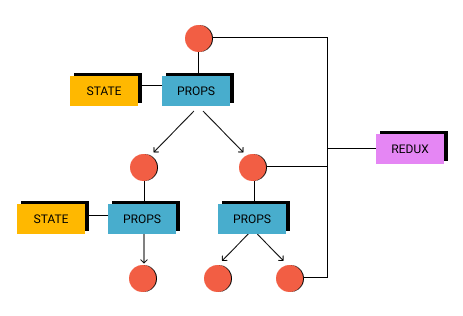
\includegraphics[scale=0.75]{./immagini/dataflow_react_redux.png}
%	}
%\end{minipage}

\section{Programmazione funzionale}
La programmazione funzionale è un paradigma di programmazione dichiarativa dove un programma è costituito dall'applicazione e dalla composizione di funzioni. In questo progetto si è utilizzata, dove possibile, la programmazione funzionale in particolare mediante le \emph{Funzioni di ordine superiore} fornite da Kotlin. Queste funzioni sono molto utili perchè permettono di scrivere codice più leggibile, conciso e soprattutto hanno la caratteristica di evitare \emph{side-effects}. Come definito dalla documentazione di Kotlin (bib: https://kotlinlang.org/docs/reference/lambdas.html), le funzioni scritte nel linguaggio Kotlin sono considerate come \emph{first-class} quindi esse possono essere contenute in variabili e strutture dati, possono essere passate come argomento di altre funzioni e possono essere ritornate da altre \emph{Funzioni di ordine superiore}. Le higher-order functions più usate nel progetto sono state:
\begin{itemize}
	\item map;
	\item sortedWith;
	\item flatMap;
	\item groupBy;
	\item more?
\end{itemize}

\section{Versionamento della soluzione}
\subsection{Git}
Git è un VCS (Version Control System) distribuito che permette di tenere traccia delle modifiche in un prodotto software e di organizzarne la codifica. In questo tirocinio è stata usata la tecnica del feature-branch: ogni aggiunta di feature corrisponde all'apertura di un nuovo branch che deve essere poi approvato previa verifica prima di essere unito al branch \verb|master|.

\subsection{Gitlab}
Gitlab è uno strumento web che permette di implementare un DevOps lifecycle che fornisce una gestione di repository git, un ITS (Issue Tracking System) e altri strumenti quali la "Continuous integration" e "Continuous deployement". Per lo sviluppo di questo progetto mi è stato fornito l'accesso al server privato aziendale Gitlab.

\section{Ambiente di sviluppo locale}
\subsection{IntelliJ Idea}
IntelliJ IDEA Community Edition è una IDE realizzata da JetBrains che fornisce funzionalità di supporto per lo sviluppo di molti linguaggi, specialmente Kotlin. Questa IDE è stata vivamente consigliata dal mio tutor aziendale per lo sviluppo in Kotlin rispetto ad altri editor per molti vantaggi come l'autocompletamento, la possibilità di eseguire un refactoring automatico di funzioni e classi e una interfacia grafica per eseguire task di Gradle.
 
\subsection{Gradle}
Gradle è uno strumento di \emph{build automation} per molti linguaggi tra cui Kotlin e Java. Gradle è stato usato per la gestione e l'installazione delle dipendenze del componente, il file di configurazione di Gradle è \verb|build.gradle.kts|, al suo interno sono definite le seguenti dipendenze:
\begin{itemize}
	\item \verb|stdlib-js|: insieme di classi e funzioni in kotlin che forniscono un entry-point per funzioni e oggetti Javascript;
	
	\item \verb|kotlin-react|: implementazione di kotlin della liberia React;
	
	\item \verb|react|: pacchetto npm della libreria React necessario per il funzionamento di \verb|kotlin-react|;
	
	\item \verb|kotlin-redux|:;
	
	\item \verb|kotlin-react-redux|:;
	
	\item \verb|kotlin-extensions|:;
	
	\item \verb|kotlinx-serialization-core|:;
	
	\item \verb|kotlinx-coroutines-core|:.
\end{itemize}
\noindent
Oltre alla gestione delle dipendenze Gradle offre delle task, utili per compilare ed eseguire l'applicativo. Nell'ambito del progetto ho utilizzato la task: \verb|runDevelopment| e come parametro della task: \verb|--continuous| in modo da eseguire automaticamente la compilazione del codice quando viene cambiato uno dei file sorgente.

\subsection{Organizzazione del lavoro}
Per l'organizzazione del lavoro, in particolare per la gestione dei macro obiettivi di ogni sprint, ho utilizzato l'ITS fornito da Gitlab che fornisce un'interfaccia Kanban che permette di categorizzare in modo efficace le singole attività da realizzare.























             % Processi
% !TEX encoding = UTF-8
% !TEX TS-program = pdflatex
% !TEX root = ../tesi.tex

%**************************************************************
\chapter{Progettazione}
\label{cap:progettazione}
%**************************************************************

%\intro{Breve introduzione al capitolo}\\
% struttura maybe?
\section{Suddivisione dei componenti grafici}
In questa sezione verranno descritti i componenti grafici e i relativi Container Redux. I componenti grafici si occupano solamente di renderizzare i dati. I container Redux si occupano di mappare lo State di Redux ai props di ogni componente in modo che essi possano accedere solo alla porzione di stato di cui hanno bisogno.
\subsection{View}
\subsubsection{TableView}
Questo componente è stato realizzato per definire la struttura generale del componente e per suddividere in modo responsivo lo spazio in quattro quadranti. Come si può vedere dalla seguente immagine ho realizzato il componente utilizzando il layout CSS Grid. Questo mi ha permesso di gestire, in modo responsivo, la struttura del componente.

\subsubsection{TableHeaderView}
Questo componente rappresenta le dimensioni superiori della tabella pivot.
Dire che la struttura della tabella è stata realizzata con flex, table, etc.

\subsubsection{TableSidebarView}
Questo componente rappresenta le dimensioni laterali della tabella pivot.
Dire che la struttura della tabella è stata realizzata con flex, table, etc.

\subsubsection{TableBodyView}
Questo componente rappresenta i dati della tabella pivot
Dire che la struttura della tabella è stata realizzata con flex, table, etc.

\subsection{Container Redux}
\subsubsection{TableController}
\subsubsection{TableHeaderController}
\subsubsection{TableSidebarController}
\subsubsection{TableBodyController}

\section{Struttura dati dell'applicazione}

\subsection{Descrizione}
Per definire lo stato dell'applicazione sono state create delle 'data class' per gestire in modo ordinato lo stato del prodotto.
\subsubsection{TableState}
Lo stato del prodotto è definito da un singolo oggetto: 'data class TableState'.
\subsubsection{UICells}
\subsubsection{TableHeader}
\subsubsection{TableHeaderAction}
\subsubsection{BodyCells}

\section{Realizzazione del JSON parser}
Lo stato dell'applicazione viene popolato in seguito ad una richiesta ad API. Queste API ritornano risultati in formato JSON. Lavorando con Kotlin non è possibile avere la stessa libertà di accesso ad un JSON come in Javascript, quindi sono stati creati delle classi per eseguire la lettura del JSON e la sua traduzione in oggetti 'data class'. GRUPPO4 ha fornito due API che dovevano essere compatibili con questo componente quindi per ognuna di esse ho realizzato un parser per trasformare un json in oggetti 'data class' e un adapter per trasformare gli oggetti data class nella data structure utilizzato nello stato dell'applicazione.

\subsection{Adapter: creavista}
Descrivi l'API\\
Descrivi il parser\\
Descrivi le funzioni\\

\subsection{Adapter: nuova interfaccia}
Descrivi l'API\\
Descrivi il parser\\
Descrivi le funzioni\\

%**************************************************************
%\section{Introduzione al progetto}

%**************************************************************
%\section{Analisi preventiva dei rischi}

%Durante la fase di analisi iniziale sono stati individuati alcuni possibili rischi a cui si potrà andare incontro.
%Si è quindi proceduto a elaborare delle possibili soluzioni per far fronte a tali rischi.\\

%\begin{risk}{Performance del simulatore hardware}
%    \riskdescription{le performance del simulatore hardware e la comunicazione con questo potrebbero risultare lenti o non abbastanza buoni da causare il fallimento dei test}
%    \risksolution{coinvolgimento del responsabile a capo del progetto relativo il simulatore hardware}
 %   \label{risk:hardware-simulator} 
%\end{risk}

%**************************************************************
%\section{Requisiti e obiettivi}


%**************************************************************
%\section{Pianificazione}             % Kick-Off
% !TEX encoding = UTF-8
% !TEX TS-program = pdflatex
% !TEX root = ../tesi.tex

%**************************************************************
\chapter{Analisi dei requisiti}
\label{cap:analisi-requisiti}
%**************************************************************
\section{Definizione delle User Stories}
Per prima cosa il team di sviluppo si è occupato di realizzare le User Stories definite mediante la seguente struttura.
\begin{longtable} {
		|>{}p{10mm}| 
		|>{}p{70mm}|
		|>{}p{15mm}|
		|>{}p{25mm}|
		>{}p{0mm}}
	\hline
	\textbf{Id} & \textbf{Descrizione} & \textbf{Priorità} & \textbf{Implementato} \\ \hline
	US1.1 & Descrizione dell'user story & A & SI \\ \hline
	\hline
	\caption{Esempio tabella User Story}
\end{longtable}
\noindent
Per ogni descrizione di un user story si possono identificare le seguenti informazioni:
\begin{itemize}
	\item \textbf{Ruolo}: definisce il tipo di utente;
	\item \textbf{Obiettivo}: definisce di che cosa ha bisogno l'utente;
	\item \textbf{Beneficio}: definisce i vantaggi che porta all'utente.
\end{itemize} 
\noindent
La sinteticità e la facilità nel definire le user story porta a vantaggi nella comunicazione tra il team di sviluppo e il cliente, rende più semplice l'aggiornamento dei requisiti e i costi di scrittura e manutenzione delle user stories sono molto bassi.

\section{Definizione del Product Backlog}
Uno dei primi obiettivi del progetto posti dal team di sviluppo è stato quello di definire il Product Backlog, cioè i requisiti del prodotto. Per ognuna delle user story precedentemente scritta è stata assegnata una priorità seguendo la seguente legenda:
\begin{longtable} {
		|>{\centering}p{10mm}| 
		|>{}p{25mm}|
		|>{}p{85mm}|
		>{}p{0mm}}
	\hline
	\textbf{A} & \textit{Priorità alta}  & funzionalità necessarie per il corretto funzionamento dell'applicazione \\ \hline
	\textbf{M} & \textit{Priorità media} & funzionalità che migliorano il prodotto \\ \hline
	\textbf{B} & \textit{Priorità bassa} & funzionalità non necessarie per il corretto funzionamento dell'applicazione \\ \hline
	\hline
	\caption{Tabella priorità User Story}
\end{longtable}
\noindent
Questo ci ha permesso di categorizzare le funzionalità principali del componente d'interfaccia grafico da quelle opzionali. Abbiamo quindi popolato il Product Backlog per ordine di \textit{priorità}, in questo modo la suddivisione delle user story per sprint, mediante le riunioni di \textit{Sprint Planning}, è stata chiara e veloce. \\
Infatti abbiamo concentrato le funzionalità principali da implementare nei primi due sprint così da avere, già a partire dal terzo sprint, un prodotto con le funzionalità principali già implementate. Dato che ogni sprint di sviluppo prevede una riunione di \emph{backlog refinement} verrano elencate tutte le iterazioni del Product Backlog.

\section{Product Backlog}
\begin{longtable} {
		|>{}p{10mm}| 
		|>{}p{70mm}|
		|>{}p{15mm}|
		|>{}p{25mm}|
		>{}p{0mm}}
	\hline
	\textbf{Id} & \textbf{Descrizione} & \textbf{Priorità} & \textbf{Implementato} \\ \hline
	US1 & Come \textbf{utente} voglio poter visualizzare i miei dati e le dimensioni relative ai dati & A & SI \\ \hline
	
	US2 & Come \textbf{utente} voglio avere una interfaccia non ostruttiva & M & SI \\ \hline
	
	US3 & Come \textbf{utente} voglio poter utilizzare questa applicazione web dal mio PC & A & SI \\ \hline
	
	US4 & Come \textbf{utente} voglio poter utilizzare questa applicazione web dal mio tablet & A & SI \\ \hline
	
	US5 & Come \textbf{utente} voglio poter utilizzare questa applicazione web dal mio telefono & A & SI \\ \hline
	
	US6 & Come \textbf{utente} voglio avere un caricamento veloce & M & SI \\ \hline
	
	US7 & Come \textbf{utente} voglio poter esplorare liberamente i dati & A & SI \\ \hline
	
\end{longtable}
\newpage
\section{Requisiti individuati dal Product Backlog}
\begin{longtable} {
		|>{}p{10mm}| 
		|>{}p{60mm}|
		|>{}p{15mm}|
		|>{}p{15mm}|
		|>{}p{15mm}|
		>{}p{0mm}}
	\hline
	\textbf{Id} & \textbf{Descrizione} & \textbf{Tipo} & \textbf{Impl.} & \textbf{User Story} \\ \hline
	
	R1.0   & \textbf{Definizione dello stato dell'applicazione} & O & SI & US1.1\\ \hline
	R1.0.1 & Sviluppo TableState        & O & SI & US1.1\\ \hline
	R1.0.2 & Sviluppo NodeDimensions    & O & SI & US1.1\\ \hline
	R1.0.3 & Sviluppo BodyCells         & O & SI & US1.1\\ \hline
	R1.0.4 & Sviluppo HeaderAction      & O & SI & US1.1\\ \hline
	R1.0.5 & Sviluppo NodeActionType    & O & SI & US1.1\\ \hline
	R1.1   & Sviluppo architettura Redux & O & SI & - \\ \hline
	R1.1.1 & Sviluppo TableStateSlice    & O & SI & - \\ \hline
	R1.1.2 & Sviluppo di Thunk & O & SI & - \\ \hline
	R1.1.3 & Sviluppo delle Actions & O & SI & - \\ \hline
	R1.1.4 & Sviluppo dei Reducers & O & SI & - \\ \hline
	
	\hline
	R2.0   & \textbf{Definizione e pianificazione dei componenti} & O & SI & US1.1\\ \hline
	R2.1   & Sviluppo dei componenti React 		  & O & SI & US1, US2, US3, US4, US5 \\ \hline
	R2.1.1 & Sviluppo di TableView                & O & SI & -     \\ \hline
	R2.1.2 & Sviluppo di TableHeaderView          & O & SI & -     \\ \hline
	R2.1.3 & Sviluppo di TableSidebarView         & O & SI & -     \\ \hline
	R2.1.4 & Sviluppo di TableBodyView            & O & SI & -     \\ \hline
	R2.2   & Sviluppo dei container Redux         & O & SI & -     \\ \hline
	R2.2.2 & Sviluppo di TableController          & O & SI & -     \\ \hline
	R2.2.3 & Sviluppo di TableHeaderController    & O & SI & -     \\ \hline
	R2.2.4 & Sviluppo di TableSidebarController   & O & SI & -     \\ \hline
	R2.2.5 & Sviluppo di TableBodyController      & O & SI & -     \\ \hline
	\hline
	R3.0   & \textbf{Sviluppo parser per JSON dell'API}         & O & SI & -     \\ \hline
	R3.1   & Sviluppo data class @Serializable 	   & O & SI & -     \\ \hline
	R3.2   & Sviluppo adapter da JSON a TableState & O & SI & -     \\ \hline
	R3.2.1   & Sviluppo funzioni XXX & O & SI & -     \\ \hline
	R3.2.2   & Sviluppo funzioni XXX & O & SI & -     \\ \hline
	R3.2.3   & Sviluppo funzioni XXX & O & SI & -     \\ \hline
	R3.2.4   & Sviluppo funzioni XXX & O & SI & -     \\ \hline
	R3.2.5   & Sviluppo funzioni XXX & O & SI & -     \\ \hline
	R3.4 & Sviluppo funzioni per effettuare richieste HTTP  & O & SI & -     \\ \hline
	\hline
\end{longtable}             % Concept Preview
% !TEX encoding = UTF-8
% !TEX TS-program = pdflatex
% !TEX root = ../tesi.tex

%**************************************************************
\chapter{Codifica}
\label{cap:codifica}
%**************************************************************

\section{Sprint di sviluppo}

\subsection{Primo sprint di sviluppo: Realizzazione della struttura dei dati e dello stato Redux}
\subsubsection{Sprint Backlog}
\subsubsection{Soluzioni implementate}
\subsubsection{Sprint Review}
\subsubsection{Backlog refinement}

\subsection{Secondo sprint di sviluppo: Realizzazione dei componenti grafici e container}
\subsubsection{Sprint Backlog}
\subsubsection{Soluzioni implementate}
\subsubsection{Sprint Review}
\subsubsection{Backlog refinement}


\subsection{Terzo sprint di sviluppo: Realizzazione del parser JSON e dell'adapter}
\subsubsection{Sprint Backlog}
\subsubsection{Soluzioni implementate}
\subsubsection{Sprint Review}
\subsubsection{Backlog refinement}


\subsection{Quarto sprint di sviluppo: Realizzazione caricamento parziale}
\subsubsection{Sprint Backlog}
\subsubsection{Soluzioni implementate}
\subsubsection{Sprint Review}
\subsubsection{Backlog refinement}



% !TEX encoding = UTF-8
% !TEX TS-program = pdflatex
% !TEX root = ../tesi.tex

%**************************************************************
\chapter{Tecnologie}
\label{cap:tecnologie-strumenti}
%**************************************************************

%\intro{Breve introduzione al capitolo}\\

%**************************************************************
\section{Kotlin}
Kotlin è un linguaggio tipizzato, realizzato da JetBrains, utilizzato da molti sviluppatori per il fatto che il codice è conciso, sicuro e permette di lavorare utilizzando librerie per la JVM, Android e il browser.

\section{React}
React è una libreria JavaScript dichiarativa, efficiente e flessibile che viene usata per costruire interfacce utente complesse da piccoli e isolati "pezzi di codice" chiamati componenti. Le principali caratteristiche che lo rendono una delle librerie più utilizzate sono la presenza di:
\begin{itemize}
	\item componenti (che possono essere scritti in modo funzionale o a classe), questo implica un alto riutilizzo del codice;
	\item virtual DOM, React crea una cache della struttura del DOM, in seguito computa le differenze e infine esegue l'update solo dei componenti che sono cambiati (riconciliazione), questo implica migliori prestazioni. 
\end{itemize}

\section{Redux}
Redux è un contenitore prevedibile dello stato per applicazioni JavaScript. Lo stato in Redux viene definito come dati che cambiano nel tempo. Lo stato determina ciò che viene renderizzato nell'interfaccia utente. Oltre alla semplice funzione di contenitore dello stato, Redux esegue anche la gestione di esso, in particolare si occupa di:
\begin{enumerate}
	\item recupero e memorizzazione dei dati;
	\item assegnare i dati agli elementi dell'interfaccia utente;
	\item modifica dei dati.
\end{enumerate}


\section{Kotlin Wrappers}
Durante la codifica del progetto sono state utilizzati alcuni wrapper forniti da JetBrains per lo sviluppo web di React, Redux e React-Redux. Questi wrapper mi hanno permesso di scrivere componenti React e utilizzare funzioni e classi delle due librerie.

\subsection{kotlin-react}
Wrapper utilizzato per l'utilizzo di funzioni che permettono la codifica di componenti React.

\subsection{kotlin-redux}
Wrapper utilizzato per la realizzazione dell'architettura Redux utilizzata nell'applicazione per la gestione dello stato.

\subsection{kotlin-react-redux}
Wrapper utilizzato per la realizzazione del collegamento tra i componenti React e lo stato di Redux.



% parlare magari di come si è scritto il codice magari

%**************************************************************
%\section{Ciclo di vita del software}
%\label{sec:ciclo-vita-software}

%**************************************************************
%\section{Progettazione}
%\label{sec:progettazione}

%\subsubsection{Namespace 1} %**************************
%Descrizione namespace 1.

%\begin{namespacedesc}
%    \classdesc{Classe 1}{Descrizione classe 1}
%    \classdesc{Classe 2}{Descrizione classe 2}
%\end{namespacedesc}


%**************************************************************
%\section{Design Pattern utilizzati}

%**************************************************************
%\section{Codifica}
             % Product Prototype
% !TEX encoding = UTF-8
% !TEX TS-program = pdflatex
% !TEX root = ../tesi.tex

%**************************************************************
\chapter{Conclusioni}
\label{cap:conclusioni}
%**************************************************************
\section{Raggiungimento degli obiettivi}
Gli obiettivi del progetto sono stati raggiunti quasi completamente. Tutti i requisiti richiesti dall'azienda sono stati soddisfatti tranne il caricamento continuo allo scroll di un utente dato i problemi riscontrati durante la codifica dello sprint numero 3.
Il componente finale è il seguente. Tutte le funzionalità previste identificate nella progettazione iniziale del progetto sono state state implementate.
%**************************************************************
\section{Conoscenze acquisite}
In questa sezione verranno identificate le conoscenze per ogni metodologia e tecnologia utilizzate nell'ambito del progetto.

\subsection{Metodologia agile}
La metodologia agile simile a SCRUM utilizzata dal team di sviluppo mi ha permesso di identificare dal punto di vista pratico le componenti necessarie a lavorare in un team di sviluppo che pratica una metodologia agile.

\subsection{Kotlin}
Durante lo studio iniziale e la codifica del componente d'interfaccia grafica mi ha permesso di arricchire la mia conoscenza del linguaggio Kotlin. Considero questa conoscenza acquisita molto importante dato che Kotlin è utilizzato da molte aziende famose tra cui: ... . Inoltre in quanto è un linguaggio che permette di realizzare molti prodotti (api, web app, applicazioni android native, etc..) penso che questo stage mi abbia fornito le basi per espandere le mie abilità su altri campi oltre che naturalmente lo sviluppo di applicazioni web.

\subsection{React e Redux}
La libreria React è utilizzata molto per la realizzazione di applicazioni web da moltissime aziende. In passato avevo già lavorato con React in progetti personali tuttavia, mediante questo progetto, penso di aver ampliato e soprattutto affinato le mie conoscenze di questa libreria. Lo stesso vale per la libreria Redux, infatti grazie allo studio e alla codifica di componenti React-Redux considero di aver migliorato e ampliato le mie conoscenze nello sviluppo web di applicazioni scalabili e manutenibili.

\subsection{Programmazione funzionale}
Lo studio delle first class functions e del loro utilizzo mi hanno permesso di entrare nel mondo della programmazione funzionale. Insieme a Kotlin e alla metodologia agile considero che queste nozioni di programmazione funzionale mi permetterranno in futuro di velocizzare la codifica e la progettazione di nuove applicazioni.

\subsection{Lavorare in un team di sviluppo}
Lavorare in un team di sviluppo mi ha fatto capire quanto importante sia la comunicazione all'interno di un progetto. Ringrazio Tobia Conforto per aver imposto un livello di comunicazione molto alto.

\subsection{Lavorare da remoto}
% forse da togliere
Dato le circostanze sociali mi sembra una skill molto importante saper lavorare da remoto.


%**************************************************************
\section{Valutazione personale}
\subsection{Effettività delle metodologie agili}
Consider l'utilizzo di una metodologia agile in un progetto software molto utile dato che il suo utilizzo permette di risolvere problemi in modo efficiente. Inoltre grazie alle sue riunioni favorisce un ambiente ricco di comunicazione che considero molto importante. La suddivisione in sprint di sviluppo, se pianificato correttamente, aiuta a mantenere il lavoro concentrato su un numero ristretto di funzionalità di un progetto e questo può aiutare per suddividere il lavoro in piccoli incrementi. Il vantaggio che ho notato maggiormente durante la codifica in sprint è stato il fatto che, dato che la struttura della metodologia agile poneva come obiettivo la realizzazione delle funzionalità più importanti nei primi sprint, questo permette di avere una visione completa di un'applicazione già dai primi sprint. 

\subsection{Effettività di Kotlin per la realizzazione di UI per il web}
Lo sviluppo in Kotlin di interfacce utente per il web è una soluzione valida ma secondo me è una tecnologia che deve maturare ancora per quanto riguarda lo sviluppo di applicazioni web.

\subsection{Effettività di React e Redux}
Molto utili, specialmente Redux che aiuta a gestire lo stato dell'appplicazione in modo molto metodico e separato dall'interfaccia grafica. Questo permette di realizzare applicazioni scalabili, un fattore molto importante specialmente nello sviluppo di applicazioni web.

\subsection{Effettività della programmazione funzionale}
L'utilizzo delle higher order function ha secondo moltissimi vantaggi per quanto riguarda la codifica di una applicazione. I vantaggi che ho identificato sono stati: aumento della velocità della codifica, aumento della leggibilità del codice durante la verifica (a causa della natura dichiarativa) e una scrittura più efficiente e concisa delle funzioni.             % Conclusioni
\appendix                               
\input{capitoli/capitolo-A}             % Appendice A

%**************************************************************
% Materiale finale
%**************************************************************
\backmatter
\printglossaries
% !TEX encoding = UTF-8
% !TEX TS-program = pdflatex
% !TEX root = ../tesi.tex

%**************************************************************
% Bibliografia
%**************************************************************
\cleardoublepage
\chapter{Bibliografia}

\nocite{*}
% Stampa i riferimenti bibliografici
\printbibliography[heading=subbibliography,title={Riferimenti bibliografici},type=book]

% Stampa i siti web consultati
\printbibliography[heading=subbibliography,title={Siti web consultati},type=online]

% !TEX encoding = UTF-8
% !TEX TS-program = pdflatex
% !TEX root = ../tesi.tex

%**************************************************************
% Ringraziamenti
%**************************************************************
\cleardoublepage
\phantomsection
\pdfbookmark{Ringraziamenti}{ringraziamenti}

\begin{flushright}{
	\slshape    
	``Life is really simple, but we insist on making it complicated''} \\ 
	\medskip
    --- Confucius
\end{flushright}


\bigskip

\begingroup
\let\clearpage\relax
\let\cleardoublepage\relax
\let\cleardoublepage\relax

\chapter*{Ringraziamenti}

\noindent \textit{Innanzitutto, vorrei esprimere la mia gratitudine al Prof. Claudio Enrico Palazzi, relatore della mia tesi, per l'aiuto e il sostegno fornitomi durante la stesura del lavoro.}\\

\noindent \textit{Desidero ringraziare con la mia famiglia per essermi stata vicina in ogni momento durante gli anni di studio.}\\

\noindent \textit{Ho desiderio di ringraziare poi i miei amici per tutti i bellissimi anni passati insieme e le mille avventure vissute.}\\
\bigskip

\noindent\textit{\myLocation, \myTime}
\hfill \myName

\endgroup


\end{document}
